% Change to use the correct class file for your paper.
\documentclass{sig-alternate-10pt}

%\pagenumbering{arabic}

%\usepackage{amsfonts}     % Adds math fonts, commands such as \begin{align}
%\usepackage{array}        % Tables for use in math mode
%\usepackage{booktabs}     % Elegant table-formatting library
%\usepackage{bold-extra}   % Provides bf+sc (only in textbf+textsc env.)
%\usepackage{bytefield}    % Formatting and layout of packets / bytefields
%\usepackage[skip=5pt]{caption}
%\usepackage{color}        % Allow the use and definition of colors
%\usepackage{colortbl}     % Color table cells
%\usepackage{comment}      % Provides \begin,\end{comment} for large blocks
%\usepackage{cprotect}     % Allows verbatim, other formatting in macro args
%\usepackage{endnotes}     % Footnotes pushed to the end of a document
%\usepackage{gensymb}      % Adds useful symbols w/out math mode, e.g. \degree
%\usepackage{graphicx}     % For importing graphics
%\usepackage{hyperref}     % Creates hyperlinks from ref/cite 
%\hypersetup{pdfstartview=FitH}
%\usepackage{listings}     % in-line source code (poorly, consider minted)
%\usepackage{mathtools}    % amsmath extension, adds more math formatting
%\usepackage{multirow}     % Multiple row spacing in tables
%\usepackage{nth}          % Typeset 33rd correctly as \nth{33}
%\usepackage[section]{placeins} % Don't let figs escape their sections
%\usepackage{rotating}     % Rotates any object, note sideways != sidewaysfigure
%\usepackage[all=normal]{savetrees} % For when space is tight, read manual and
                          % selectively enable things. CAN BREAK CONF STYLES!!
%\usepackage{soul}         % Provides \hl{} for highlighting
%\usepackage{subfig}
%\usepackage{subfigure}    % Complicated figure creation
%\usepackage{subcaption}   % Replaces both subfig and subfigure
%\usepackage[nofancy]{svninfo} % svn information in docs (req. svn:keywords)
%\usepackage{tabularx}     % Complicated table creation
%\usepackage{threeparttable} % Add footnotes to a table
%\usepackage{units}        % For nice fractions, \nicefrac{1}{2} --> 1/2
%\usepackage{url}          % Pretty printing of hyperlinks
%\usepackage{xspace}       % Intelligently add spaces after commands

%%%%%%%%%%%%%%%%%%%
%%% new package %%%
%%%%%%%%%%%%%%%%%%%
\usepackage{epsfig,xspace,multirow,capt-of,comment}
\usepackage[hyphens]{url}
\usepackage{hyperref}
\usepackage[hyphenbreaks]{breakurl}
\usepackage{graphicx,amssymb,amsmath,endnotes}
\usepackage{times}
\usepackage{subfigure}
\usepackage{ulem}
\usepackage{rotating}
\usepackage{wasysym, pifont}
\usepackage[usenames,dvipsnames]{color}
\usepackage{placeins}
\usepackage{balance}
\usepackage{epstopdf}
\epstopdfsetup{update}
%%%%%
% used in QxDM section
\usepackage{algorithmic}
\usepackage{algorithm}
\usepackage{array}
\usepackage{tabularx}
\usepackage{enumitem}

%%%%%
% used in QxDM section
\usepackage{algorithmic}
\usepackage{algorithm}
\usepackage{array}
\usepackage{tabularx}
%%%%%
% convert eps to pdf
\usepackage{epstopdf}
\epstopdfsetup{update}
%%%%%

\usepackage{epsfig,xspace,multirow,capt-of}
\usepackage{hyperref}
\usepackage{graphicx,amssymb,amsmath,endnotes}
\usepackage{times}
\usepackage{ulem}
\usepackage{rotating}
\usepackage{wasysym, pifont}

%\DeclareCaptionType{copyrightbox}

\newlength\SUBSIZE

\renewcommand{\arraystretch}{1.2} % Space out rows in tables

%\setlength\paperheight {11in}
%\setlength\paperwidth {8.5in}

\hyphenpenalty=800
\tolerance=400

% italics for bibliography
\normalem


%%%%%
% new command
\newcommand{\MR}[1]{\multirow{2}{*}{#1}}

\newcommand{\mysection}[1]{\vspace{-.07in}\section{#1}\vspace{-.02in}}
\newcommand{\mysubsection}[1]{\vspace{-.05in}\subsection{#1}\vspace{-.02in}}
\newcommand{\mysubsubsection}[1]{\vspace{-.05in}\subsubsection{#1}\vspace{-.02in}}


\newcommand{\hd}[1]{\small{\textbf{\texttt{#1}}}\normalsize}
\newcommand{\hds}[1]{\small{\textbf{\texttt{#1}}}}
\newcommand{\hdf}[1]{\small{\textbf{\texttt{#1}}}\footnotesize}

\newcommand{\ISP}{$\sf\small{ISP}$}
\newcommand{\ISPP}{$\sf\small{ISP}$ }
\newcommand{\UMICH}{$\sf\small{UMICH}$}
\newcommand{\UMICHH}{$\sf\small{UMICH}$ }

\newcommand{\YY}{\CIRCLE}
\newcommand{\NN}{\Circle}
\newcommand{\YN}{\RIGHTcircle}
\newcommand{\XX}{\ding{53}}

\newcommand{\Ignore}[1]{{\small }}
\definecolor{gray}{rgb}{0.5,0.5,0.5}
\newcommand{\etc}{\emph{etc.}\xspace}
\newcommand{\ie}{\emph{i.e.,}\xspace}
\newcommand{\eg}{\emph{e.g.,}\xspace}
\newcommand{\etal}{\emph{et al.}\xspace}
\newcommand{\wrt}{\emph{w.r.t.}\xspace}
\newcommand{\aka}{\emph{a.k.a.}\xspace}
\newcommand{\AlgBox}[1]{{\framebox[1.2\width]{\textbf{#1}}}}

\renewcommand{\paragraph}[1]{\smallskip\noindent{\bf{#1.}}}
\newcommand{\paragrapha}[1]{\smallskip\noindent{\bf{#1}}}
%\renewcommand{\algorithmiccomment}[1]{//#1}

\makeatletter
  \newcommand\figcaption{\def\@captype{figure}\caption}
  \newcommand\tabcaption{\def\@captype{table}\caption}
\makeatother

\newcommand{\vsp}{\vspace{+0.15in}}

\newcommand{\nsection}[1]{\vspace{-1em}\section{#1}\vspace{-0.7em}}
\newcommand{\nsubsection}[1]{\vspace{-0.85em}\subsection{#1}\vspace{-0.55em}}
\newcommand{\nsubsubsection}[1]{\vspace{-0.4em}\subsubsection{#1}\vspace{-0.3em}}
\newcommand{\ncaption}[1]{
 	\vspace{-1.2em}
	\caption{#1}
% 	\vspace{-1.5em}
}
%%%%%


\begin{document}

\title{Fast Re-Tx: Mobile Latency Optimization with Cross Layer Analysis}

% AUTHOR STYLE 1
\author{
 \alignauthor{Haokun Luo}\\
 \affaddr{University of Michigan}\\
 \email{\{haokun\}@umich.edu}
}

\conferenceinfo{EECS 582 -- Winter'13} {Jan 10--Apr 23, 2013, Ann Arbor, Michigan, USA.}
\CopyrightYear{2013}

\maketitle

\begin{abstract}
% ABSTRACT

Slow network experience on smartphone could hurt user experience and downgrade application reputation. When users are urgent about specific information, the carried information size is small but the latency of the mobile network service is very sensitive. The discontinuous burst of short data transmission is the most common traffic pattern in the cellular network. But significant latency appears at the beginning part of the data transmission. In order to identify the root cause, I use diagnostic cross layer monitoring tool, QxDM (Qualcomm eXtensible Diagnostic Monitor), and found that inactive response to packet loss in the RLC (Radio Link Resource) leads to unnecessary timeout in the transport layer. I propose a RLC \textit{Fast Re-Tx (Retransmission)} mechanism to avoid sluggish reaction to packet loss, and further reduce the latency during the initial network connection. Based on our simulation results, the \textit{Fast Re-Tx} mechanism could reduce the latency by up to \textit{35.69\%} over initial network connection.


\end{abstract}


\terms{Mobile, Measurement}
\keywords{RRC state machine, Cross Layer Analysis, RLC Fast Retransmission, Latency Optmization}

%\newpage

% page limit          % 14.0 pg
% abstract            %  0.5 pg
%\vfill\eject
\section{Introduction}

% UMTS Network

% RRC State Machine
3G cellular data networks have recently witnessed rapid growth, especially due to the emergence of smartphones. In this paper, we focus on the\textit{ Universal Mobile Telecommunications System} (UMTS) 3G network, which is among the most popular 3G mobile communication technologies. However, the bottleneck of the internet resides in the first hop of the network, and large amount of lower layer retransmission could cause significant latency~\cite{bufferbloat}. 3G network has a bad reputation at the initial period of network connection~\cite{3g.slow}, and significant delay will hurt user experience badly. In this paper, we are going to allocate the fundamental cause of the abnormal latency, and propose a modified protocol solution.

3G network systems operate under radio resource constraints. To efficiently utilize the limited radio resources, UMTS introduces for each \textit{user equipment} (UE, i.e. smartphone) a \textit{radio resource control} (RRC) state machine, such as in Figure~\ref{fig:rrc.state.machine}, that determines radio resource usage affecting device energy consumption and user experience~\cite{spec-3G-RRC}. UE will stay in one of three states, each with different amount of allocated radio resources. The transitions between states also have significant impact on the UMTS system.

\begin{figure}
\centering
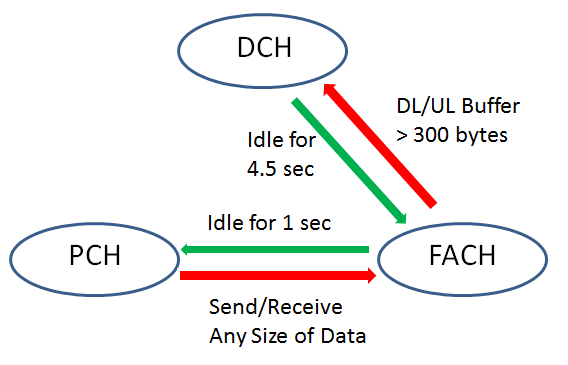
\includegraphics[width=0.45\textwidth]{figs/rrc_state.png}
\caption{RRC State Machine for the 3G UMTS network for T-Mobile}
\label{fig:rrc.state.machine}
\end{figure}

The network topology provides a nature isolation between different layers. The design of transport layer protocol doesn't require the knowledge of lower layer information. However, the abstraction of the design could lead to sub-optimal scenario, i.e. large significant latency will occur during the RRC state transition. Since the root cause of the abnormal delay behavior resides in the data link layer (i.e. RLC, radio link control, layer), the visibility of lower layer information will help us identify the root cause of the bizarre behavior in upper layer. 

Previous studies~\cite{3g_rrc, 4g_rrc, aro, opt.tcp.rlc} don't have accessibility to detailed link layer data transmission information, so they have to treat the lower layer as a black box, and use inference technique to determine and control RRC states with less accuracy. In our study, the QxDM tool is able to capture the fine grained data transmission and context information (i.e. signal strength, RLC protocol configuration) in both upper and lower layers. To the best of our knowledge, our study is the first cross-layer analysis that have both ground truth knowledge in transport layer and data link layer. Thanks to our cross-layer visibility, we identify the root cause of the unexpected latency as the RLC protocol's lagging response to the packet loss signal. We propose \emph{Fast Re-Tx} as the improved RLC layer mechanism to reduce the latency over the initial data transmission. We summarize our contributes here:

\begin{itemize}
\item \textbf{Novel cross-layer mapping mechanism to fully correlate multiple network layers.} We develop the first cross-layer mapping algorithm that accurately maps the TCP/UDP packets to the corresponding \textit{packet data unit} (PDU) in the RLC layer. Our mapping accuracy is on average 99.8\%.
\item \textbf{Root cause analysis on the performance issue and propose feasible solutions.} Based on the cross-layer mechanism, we could perform an in-depth analysis on RLC layer behavior during the initial data transmission period. We found that the RLC sender doesn't reactive to PDUs loss signal --- duplicate \textit{acknowledgement} (ACK) PDUs, and it leads to upper layer packet delays, and even TCP \textit{retransmission timeout} (RTO). Therefore, we propose RLC \emph{Fast Re-Tx} to actively respond to duplicate RLC ACK PDUs to reduce the latency over problematic initial data transmission period. We evaluate the improved mechanism using real time traces, and estimate the RLC \textit{round-trip time} (RTT) could drop up to 35.69\% over FACH state.
\end{itemize}

%Therefore, cross-layer analysis over QxDM logs would help us have a in-depth understanding the correlation between different layers, and identify the root cause of abnormal latency behaviors during the initial state of data transmission.

%\begin{figure}
%\centering
%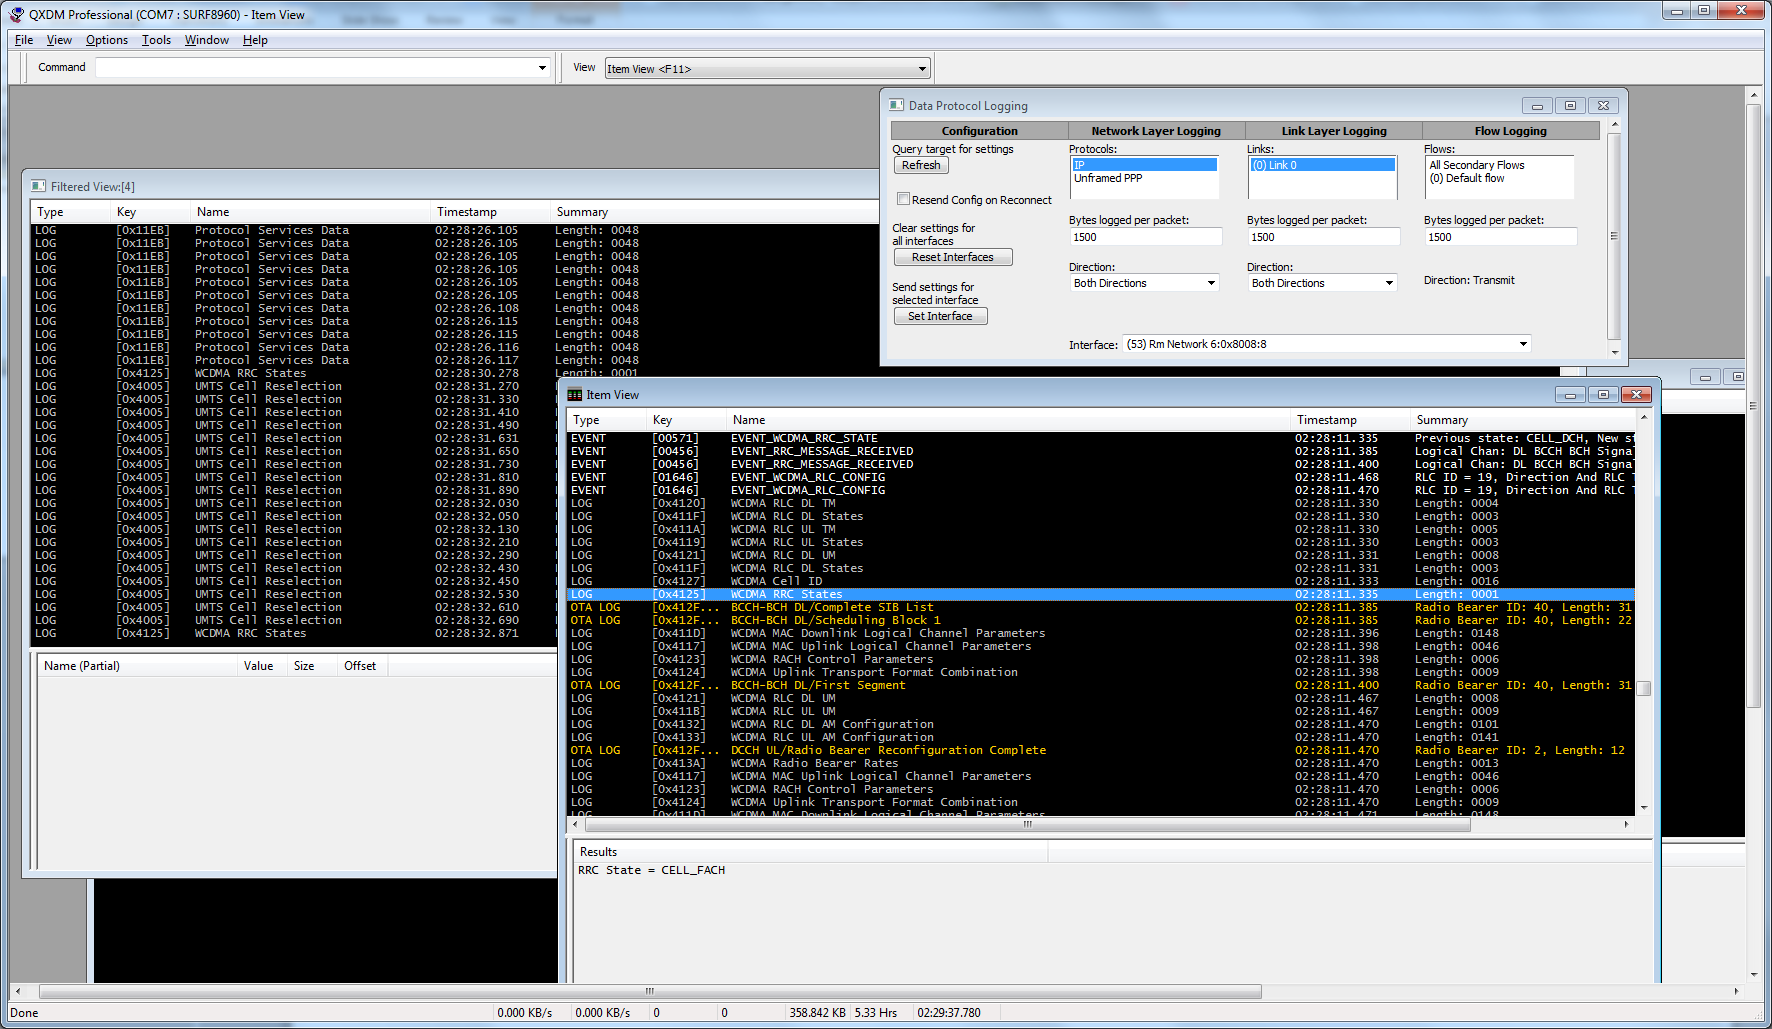
\includegraphics[width=0.45\textwidth]{figs/QxDM.png}
%\caption{Ongoing monitoring and logging activities on QxDM}
%\label{fig:qxdm}
%\end{figure}

\label{sec:intro}

         % 1.5 pg
\input{background}
%\clearpage
%\section{Measurements}

\subsection{RRC State Inference}
The previous RRC state inference study provides a decent methodology to infer the RRC state machines~\cite{3g_rrc}. They want to infer the DCH demotion timer and FACH demotion timer in the RRC state machine. The methodology is to send a MAX (1024) bytes size packets to let the handset promote to DCH. Then wait for various amount of times (or called gap periods) to allow the handset stay in DCH, or demote to FACH, or even further demote to PCH. And send another packet with size of Max or Min (30) bytes. They measure the RTT (Round Trip Time) delay for each fixed gap period. They will infer the demotion timer by observing a larger RTT difference between two consecutive pre-defined gap periods. For example, if the RTT at gap period of 4 s is 3 times larger than that of 3.5 s, then they will conclude the FACH demotion timer is around 4 s. Since the handset will demote to FACH and promote to DCH (sending another packet) again at 4 s, the extra state transition delay contributes to the larger RTT. I repeat their experiments using UDP packets, and let the server respond an echo packets once the transmitted packet get received. In Figure~\ref{fig:rrc.infer}, I could observe an unexpected delay over FACH initial state and FACH to DCH promotion transitions, which implies the latency that mobile user could experience during the initial stage of data transmission.

% RLC Loss ratio per RRC state
\begin{figure}
\centering
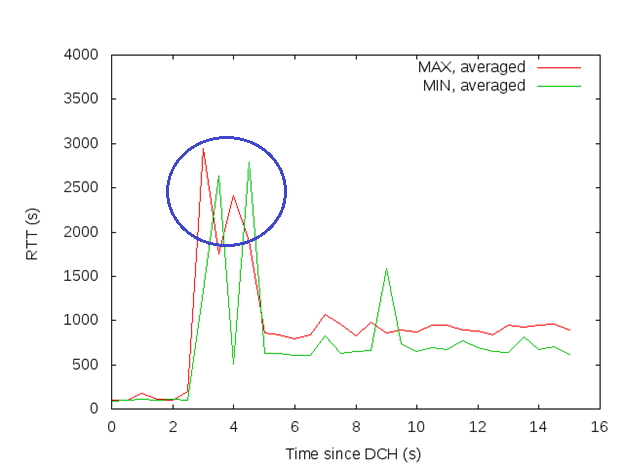
\includegraphics[width=0.45\textwidth]{figs/rrc_infer.png}
\caption{Unexpected large RTT during initial part of FACH state and FACH to DCH promotion transition}
\label{fig:rrc.infer}
\end{figure}

\subsection{Control Experiments}

% UDP/ TCP control experiment set up
The purpose of the control experiments is to verify the unexpected delays over noisy FACH state, and identify the root cause of the problem. First, we repeated our active RRC inference test for 160+ hours and dump both the client QxDM and server side tcpdump traces to perform offline analysis~\cite{tcpdump}. In order to distinguish the identities of each UDP packets, we manually injected a "sequence number" into the first four bytes of the sender's randomized payload, and the echo server sent back the received sequence number as acknowledge number in its payload. I refer the trace as \emph{UDP\_{}Trace}. Second, we designed a packet train probing using TCP packets so that we could recreate the "pseudo-state" issue~\cite{pkt.train}. Basically, we send a "train" of TCP packet size of 10 KB bytes with interleaving gap period of 3 seconds to 5 seconds incremented by 0.5 seconds with the total of 500 packets. The gap period is the DCH demotion timer period considering the variance in the lossy channel, and adjacent packet will transmit the packet starting from FACH state. Therefore, we will have more transition over the troublesome FACH state to allow us to take a closer look the root cause. Since TCP has its own ARQ (automatic repeat request) mechanism, it would be interesting to investigate the RLC retransmission's delay influence over TCP retransmission. I will refer the trace as \emph{TCP\_{}Trace}.

\label{sec:measure}

         % 3.0 pg
\input{observation}
\input{methodology}
%\section{Cross Layer Analysis}

This section briefly describes the how I collect ground truth data transmission information in IP and RLC layer using QxDM in subsection 1. Subsection 2 talks about the core algorithm to enable cross layer mapping. Subsection 3 verifies the latency observations using cross layer algorithm. Subsection 4 describes about how I calculate the RLC retransmission ratio in QxDM. Subsection 5 identifies the root cause of latency by results from both emph{UDP\_{}Trace} and emph{TCP\_{}Trace}, and propose RLC \textit{Fast Re-Tx} mechanism to reduce the RLC delay.

\subsection{QxDM Tool}

% Describe what the tool does
QxDM is a real-time data collection and diagnostic logging tool for measuring mobile-based RF (Radio Frequency) performance~\cite{qxdm_flyer}. It is a Windows based monitoring application. When I perform control experiments and real application measurements, I plug in the device to the desktop or laptop with QxDM software installed. Once the experiments finishes, I filtered out the real-time monitoring information related to IP packets, RLC PDUs (protocol data unit, the smallest data transmission unit in RLC layer), and RRC states in Table~\ref{tab:QxDM.logs}, and dump the results into a log file. The 0x11EB log entry includes IP headers, IP payloads, and its customized header. Since large IP packets will be fragmented into smaller segments, the customer header could indicate the segment index of the whole IP packet. The 0x4132 and 0x4133 unveil the RLC AM (acknowledge mode) configurations, i.e. the polling function timers, the retransmission limit for a single PDU, and etc. The 0x413B, and 0x418B provides RLC PDU header and first byte payload information for both data PDUs and control PDUs (or STATUS PDUs) in both uplink and downlink directions. We wrote a QxDM log parser to aggregate the filtered entries, and apply cross layer analysis to understand the correlation between different layers. I conduct all the experiments on two devices -- Galaxy S3 with Android OS 4.1.1 and HTC One S with Android OS 4.0.4, to observe any device dependent behavior.

%QxDM provides precise RRC state information to indicate the current radio channel state. RLC data PDU and status PDU will assist us in cross layer mapping to the transport layer data, i.e. TCP/UDP. Other context information could also be found in the log, i.e. signal strength and physical layer transmission bit rate. The QxDM log is essentially a list of log entries formatted as a uniformed header with timestamp, a detailed log entry description, and a raw hex dump result.  

% Table of QxDM entries
\begin{table}
\begin{tabularx}{0.48\textwidth}{ | c | X | }
	\hline
  	\textbf{QxDM Log ID} & \textbf{Description} \\
  	\hline\hline
  	0x11EB & IP data packets \\
  	\hline
  	0x4132 & WCDMA RLC downlink acknowledge mode configuration \\
  	\hline
  	0x4133 & WCDMA RLC uplink acknowledge mode configuration \\
  	\hline
  	0x413B & WCDMA RLC uplink acknowledge mode PDU \\
  	\hline
  	0x418B & WCDMA Flexible RLC downlink acknowledge mode PDU \\
  	\hline
  	0x4125 & WCDMA RRC states \\
  	\hline
\end{tabularx}
\caption{QxDM log entries used in cross layer analysis}
\label{tab:QxDM.logs}
\end{table}

% UDP results
\subsection{Verification Latency in QxDM}

% UDP loss behavior over different states
QxDM provides the ground truth information about RRC state, so I want to validate the delay behavior based on the inferred RRC model. To verify the packet delay in the transport layer over each RRC state, I need to know the RRC state for transport layer packets and RLC layer PDUs. Since each RRC state log is only a single log entry indicating the change of RRC state, I don't have explicit RRC state information tied to each packet and PDU. Therefore, I determine the RRC states by backtracking the most recent RRC state log, then assign as attributes to the packets and PDUs so that I could acquire RRC state information directly from the packet or PDU itself. 

Because the the promotion period for PCH and FACH differs from their initial period due to additional signaling overhead, I want to distinguish between a RRC state with and without involving transitions. Since I focus on the initial period of data transmission, the RRC state promotion is more meaningful than state demotion, which is the end of whole data transmission period. So RRC state promotion is our preliminary concern for this project. We break down the normal FACH into FACH\_{}INIT and FACH\_{}PROMOTE states. Similarly, PCH was divided into PCH\_{}INIT and PCH\_{}PROMOTE. Since the FACH promotion timer is around 2 seconds and PCH promotion state is around 0.5 seconds. I define the FACH\_{}PROMOTE state as the time slot of counting back 2 seconds from the point of promoting to DCH. For the same reason, PCH\_{}PROMOTE state describes the time slot of counting back 0.5 seconds from the point of promoting to FACH. 

From the \emph{UDP\_{}Trace}, I calculate the UDP RTT by mapping the client transmitted UDP packets to the served echoed back packets through comparing the manually injected "sequence number". If both packets have the identical "sequence number" in their first four byte payload, then the RTT for the transmitted data is the timestamp difference between the two packets. Figure~\ref{fig:udp.rtt} shows the UDP RTT broken down into different RRC state and state transitions. The average RTT at FACH\_{}INIT state is \textit{2.52 s} for HTC One S and \textit{2.08 s} for Galaxy S3, which around both around \textit{190\%} greater than each one's RTT in DCH. The average RTT for FACH\_{}PROMOTE state is \textit{1.14 s} for HTC One S and \textit{1.05 s} for Galaxy S3, which are around \textit{40\%} greater than those in DCH. The result could validate the abnormal delay behavior especially during the initial part of the FACH state, namely the FACH\_{}INIT state. We could also observe a tremendous latency over PCH\_{}PROMOTE state. Because packets cannot stay in PCH during the transmission, the promotion to FACH and DCH will double the signaling overhead, which introduces more latency.

% UDP delay
% RLC Loss ratio per RRC state
\begin{figure}
\centering
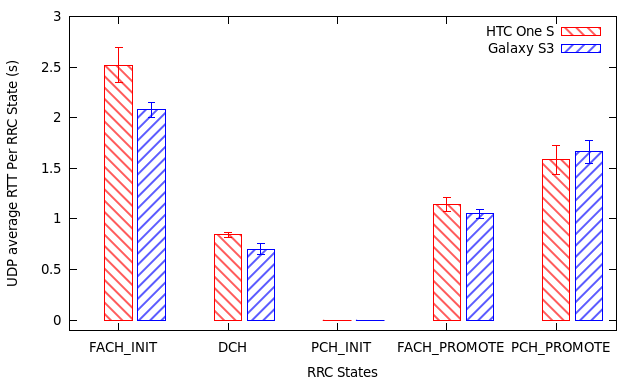
\includegraphics[width=0.45\textwidth]{figs/udp_rtt.png}
\caption{UDP RTT calculated from the QxDM log result}
\label{fig:udp.rtt}
\end{figure}

\subsection{Cross Layer Algorithm}

% Describe the mapping algorithm I use for cross-layer analysis
QxDM tool provides fine grained lower layer RLC layer transmission information. If I could correlate the transport layer packets with the RLC layer transmitted PDUs, I will have a transparent view of the link layer behaviors, especially the RLC retransmission. One of the fundamental limitation of QxDM is the partial logging issue. For example, only the header and first byte data payload will be logged for each RLC PDU. It is also possible that a small fraction of RLC PDUs cannot be captured, which lead to a unnecessary sequence number gap. Our mapping algorithm will handle all the limitations I have mentioned.

% The mapping algorithm here
The cross layer mapping algorithm is essentially a map between the complete IP packets (known as SDU) and corresponding fragmented RLC payload data bytes (known as PDU). Due to the partial logged information in QxDM, only the first data byte is captured in the log. Thus, I have to skip over the rest of the PDU, and try to match for the first data byte in the next PDU. The problem at this point is to determine the end of IP packets while I iterate through the consecutive RLC PDUs. Since each PDU could either contain the payload data dedicated to a single SDU or belongs to two SDUs. If the reminder size of the SDU cannot fulfill the largest size of PDU, then RLC protocol will concatenate the part of the next SDU to fill the rest of space~\cite{spec-3G-RLC}. Ultimately, if the accumulative mapped index equals the size of SDU, I claim to find a mapping successfully; otherwise no mapping discovered. Algorithm~\ref{alg:cross.mapping} states the detailed information of the mapping mechanism.

% the corner case of the mapping algorithm
There is a corner case in the mapping algorithm such that the QxDM cannot capture the some of the SDUs. Similar to TCP protocol, the sequence number in RLC PDUs could uniquely distinguish between every PDUs. If there are some missed PDUs, then I cannot map the first byte data for every PDU size. In that case, I could even skip over the missed PDUs and add up multiple of PDU size to hunt for a match, which is represented as "factor" variable in the mapping algorithm. However, the aggressive leap mapping mechanism cannot fully recover the corner case, especially when the missed PDUs were either the beginning or the end part of the mapped RLC list. I evaluate the improved mapping algorithm by checking the percentage of mapped IP packets in all the traces of control experiments, and the average mapping ratio is \textit{99.8\%}.

% algorithm detail
\begin{algorithm}
\begin{algorithmic}
\STATE {\textit{\textbf{Function} isCrossLayerMapped(SDU, PDU\_{}list):}}
\STATE {\textit{PDU\_{}index} = $0$}
\STATE {\textit{SDU\_{}byte\_{}index} = $0$}
\WHILE {\textit{SDU\_{}byte\_{}index} $<$ size of \textit{SDU}}
\IF {\textit{SDU[SDU\_{}byte\_{}index]} == \textit{cur\_{}PDU}}
	\STATE {\textit{cur\_{}PDU} = \textit{PDU\_{}list[PDU\_{}index]}}
	\STATE {$factor$ = \textit{cur\_{}PDU}.sn - \textit{last\_{}PDU}.sn  // sn is sequence number}
	\STATE {\textit{last\_{}PDU} = \textit{cur\_{}PDU}}
	\IF {\textit{cur\_{}PDU} has LI field in header}
		\STATE {Increase \textit{SDU\_{}byte\_{}index} by the value of LI field}
	\ELSE
    		\STATE {Increase \textit{SDU\_{}byte\_{}index} by the size of \textit{cur\_{}PDU} multiples $factor$}
    	\ENDIF
    	\IF {\textit{cur\_{}PDU}'s HE field is $2$}
    		\STATE {Break}
    \ENDIF
    	\STATE {Increase \textit{PDU\_{}index} by $1$}
\ELSE
	\STATE {Break}
\ENDIF
\ENDWHILE
\IF {\textit{SDU\_{}byte\_{}index}== size of \textit{SDU}}
	\RETURN \TRUE
\ELSE
	\RETURN \FALSE
\ENDIF
\end{algorithmic}
\caption{Decide whether one TCP/UDP packet maps to all corresponding RLC PDUs}
\label{alg:cross.mapping}
\end{algorithm}

\subsection{RLC Retransmission Calculation}

The RLC layer retransmission is a protection mechanism that maximize the reliability over a loss data transmission channel. However, it also causes the delays due to duplicate transmissions without noticing the upper layers. To assist further identifying the root cause of the latency, we first introduce how we calculate the RLC retransmission from the QxDM logs.

% how to calculate the RLC retransmission
The sequence number of the RLC PDU will uniquely identify each RLC packet. Therefore, I determine the RLC retransmission based on the duplicate of sequence numbers. Since the size of RLC PDU is only 42 bytes and is very limited, if the RLC keeps an effective throughput, it has to reduce the number of bits in the header to hold the sequence number. Therefore, the sequence number only consumes 12 bits (range of 0-4095) in the current RLC protocol~\cite{spec-3G-RLC}. As a result, sequence number is circularly reused every 4096 PDUs, and it is always increasing. To avoid over-count the duplicate sequence number in different cycle, I hard set a smaller window size of 512 to count the reappearing sequence number within that range. I determine the RRC state for each RLC PDU by backtracking to most recent RRC state log entry, and fetch the RRC state based on that log content. I break down RLC retransmitted PDUs based on their RRC states, and I calculate the retransmission ratio through dividing total number of retransmitted PDUs per RRC state by the total number of PDUs in that RRC state. 

\subsection{Root Cause Analysis and Solutions}

% explain why I want to calculate RLC layer retransmission and how to calculate
There are two possible behaviors of RLC retransmission that leads to transport layer delay. The first one is that retransmission is necessary because of noisy channel during FACH state. Based on \emph{UDP\_{}Trace}, I could see a strong correlation between RLC retransmission ratio and FACH state as an evidence. One possible solution is that application could batch the data transmission to reduce the RRC state promotion frequency~\cite{3g_rrc}. The second one is the retransmission get unnecessary delayed caused by the lagging response to the PDU loss signal. I observe it from \emph{TCP\_{}Trace} when I studied the relationship between TCP retransmission and RLC retransmission. I will also provide a improved RLC mechanism to avoid the unnecessary delay later.

% UDP trace analysis
Analyzing the \emph{UDP\_{}Trace} based on the RLC retransmission calculation methodology, we calculate the RLC retransmission ratio per RRC state in Figure~\ref{fig:RLC.Loss.Per.RRC.UDPTrace}. As we can see, the RLC retransmission among FACH and FACH\_{}PROMOTE in total are \textit{53.46\%} for HTC One S device with standard deviation of \textit{4.58\%}, and \textit{13.74\%} for Galaxy S3 devices with standard deviation of \textit{1.14\%}. It strongly suggested the significant delay over the FACH\_{}INIT and FACH\_{}PROMOTE states, which indicates the higher chance of RLC retransmission in a resource shared and noisy channel during FACH state. We could also observe that the HTC device has a higher loss rate than that of Galaxy S3. One possible explanation for device dependent behavior is that the difference in hardware module. The HTC One S was produced over Snapdragon S3 MSM8260, while the Galaxy S3 contains Snapdragon S4 MSM8960, which is the next generation of the one for HTC One S. The wireless radio techniques for Snapdragon S4 has support for larger range of network types~\cite{snapdragon}. The detailed discussion about the hardware differences is out of the scope of this paper.

% RLC Loss ratio per RRC state
\begin{figure}
\centering
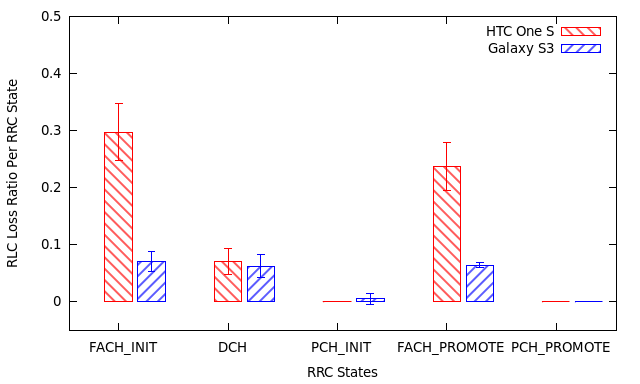
\includegraphics[width=0.45\textwidth]{figs/rlc_retx_udp.png}
\caption{Significant RLC retransmission ratio over stable FACH state and FACH promotion state strongly implies the upper layer latency during the beginning part of the data transmission}
\label{fig:RLC.Loss.Per.RRC.UDPTrace}
\end{figure}

%TCP Trace Analysis
TCP retransmission timeout (RTO) could cause apparent round trip delay due to congestion window drop by half and restarting the data transmission from the slow start phase~\cite{tcp.rto}. From the \emph{TCP\_{}Trace}, I correlate the TCP retransmission behavior with the RLC retransmission through our mapping algorithm. By capturing the root cause of the TCP RTO, I found that current RLC protocol has a sluggish response to the PDU lost signals -- the duplicate ACKs, in Figure~\ref{fig:RLC.Dup.Ack}. The delayed RLC retransmission PDUs leads TCP RTO, which further introduces latency in the transport layer. In 3GPP RLC specification, the sender only retransmits the PDU once it receives the STATUS LIST (or non-acknowledged) control PDU from the receiver, but ignores to duplicate ACKs, which is a strong hint for PDU loss~\cite{spec-3G-RLC}. If we could bring the group of retransmitted RLC PDUs from 2.8 s to 0.5 s, then we could avoid TCP RTO, reducing the latency more than 2.3 s. Therefore, I propose a RLC \textit{Fast Re-Tx} mechanism, which will retransmit the unacknowledged PDUs once the sender receives three duplicate RLC PDU ACKs. The faster reaction to loss signals could reduce RLC layer latency and further reduce the latency in transport layer.

% explain the root cause of the longer delay analysis
\begin{figure}
\centering
% DON'T add file extension for .eps images
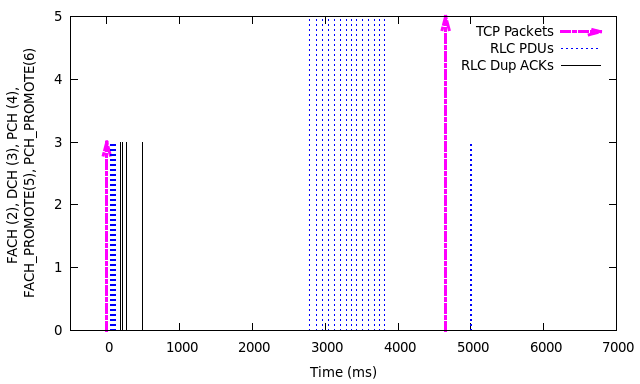
\includegraphics[width=0.45\textwidth]{figs/rlc_dup_ack.png}
\caption{Two Latency Causes: short DCH demotion timer and lagging response to the PDU lost signal}
\label{fig:RLC.Dup.Ack}
\end{figure}

\label{sec:crossAnalysis}



\input{rootCauseAnalysis}
\section{Evaluation}

\subsection{RTT Estimation}
We first define the RTT in RLC layer. In the RLC protocol, the STATUS PDUs (ACK or NACK) don't generate by every received RLC PDU, but triggered either by receiving a polling request from the sender or by detecting one or more missed PDUs from its receiver buffer~\cite{spec-3G-RLC}. Since the QxDM traces are collected at the client side, we don't have the information of when the server side receive the PDU. Thus, I estimate the RTT of a RLC PDU based on the timestamp difference between the most recent sender's polling request and received ACK. Based on RLC configuration, the maximum polling request frequency is 500 ms. One of the previous mobile RTT estimation study shows the autocorrelation coefficient of two RTT measurements within 500 ms is more than 0.6~\cite{proteus}. Therefore, my estimation is still reasonable to be considered as the real RLC RTT value.

\subsection{Cost-Benefit Analysis}
In order to know whether the new proposed RLC mechanism works, I apply a cost-benefit analysis over the existing \emph{TCP\_{}Trace}. The definition of benefit and cost is straight forward. Basically, if the fast retransmitted PDUs will be transmitted in the future, then we compare the RTT if it transmitted right after the duplicate ACKs with the real RTT value in the trace. If the difference is less than 0, we call that is a benefit. In the same way, if it is greater than 0, we call it a cost. However, we want to know if the PDU is really lost over the channel, or it just gets delayed due to channel contention. That depends on whether the sender receives a ACK or NACK (a list of unreceived PDU sequence numbers). We categorize the situations into four cases -- Win, Draw\_{}Plus, Draw\_{}Minus, and Loss. If the sender will receive a NACK, and more than 50\% of the fast retransmitted PDUs will retransmit in the real trace, then we call the case "Draw\_{}Plus" as in Figure~\ref{fig:draw.plus}. Since it would brings us benefit if the fast retransmit RTT is less than the RTT in the real trace. The "Win" case is defined that if we could avoid a TCP RTO based on the "Draw\_{}Plus" in Figure~\ref{fig:win}. In that case, RLC layer benefit is the same as "Draw\_{}Plus", but I want to highlight that it could bring further latency benefit over the transport layer. "Draw\_{}Minus" occurs when less than 50\% of the fast retransmitted PDUs get really retransmitted in the real trace as in Figure~\ref{fig:draw.minus}. If the sender gets a ACK with a larger sequence number, then all the PDUs were successfully delivered to the receiver. In that case, we called the case "Loss", since all the retransmitted packets are redundant as in Figure~\ref{fig:loss}. 

As we can see from Table~\ref{tab:rlc.fast.sim}, around 75\% of the time we will have benefit on RLC latency reduction if we count the "Win" and "Draw\_{}Plus". The overall RLC delay could be reduced by \textit{2.66\%} over all the RRC state based on trace simulation analysis. If we break down the cost-benefit over different RRC states, the RLC RTT latency could reduce by up to \textit{35.69\%} over initial FACH state or FACH promotion transitions. Therefore, we could have a large latency benefit over the initial period of data transmission.


% Four cases
\begin{figure}
\centering
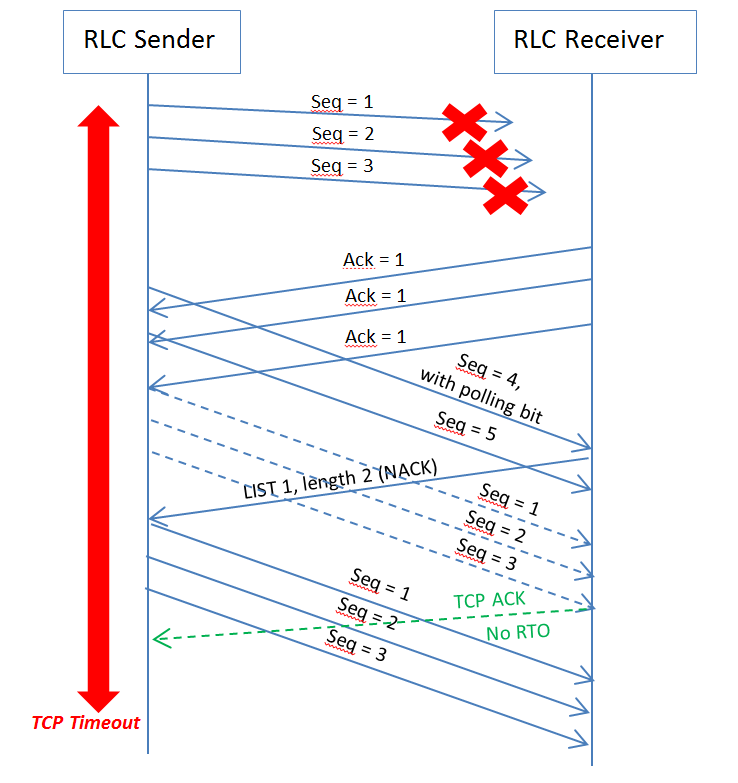
\includegraphics[width=0.45\textwidth]{figs/Win.png}
\caption{Win: RLC Fast Re-Tx avoid a TCP RTO}
\label{fig:win}
\end{figure}

\begin{figure}
\centering
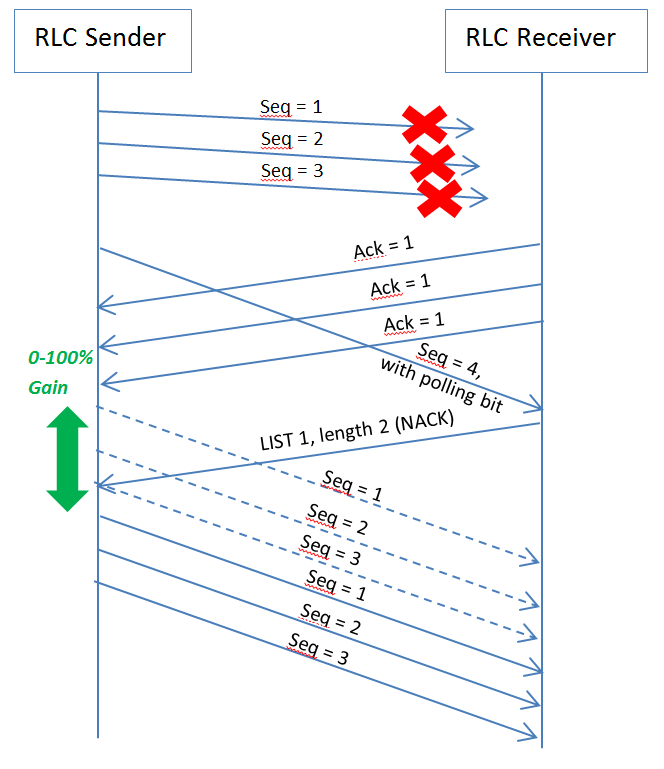
\includegraphics[width=0.45\textwidth]{figs/Draw_plus.png}
\caption{Draw Plus: the predication accuracy is more than 50\%}
\label{fig:draw.plus}
\end{figure}

\begin{figure}
\centering
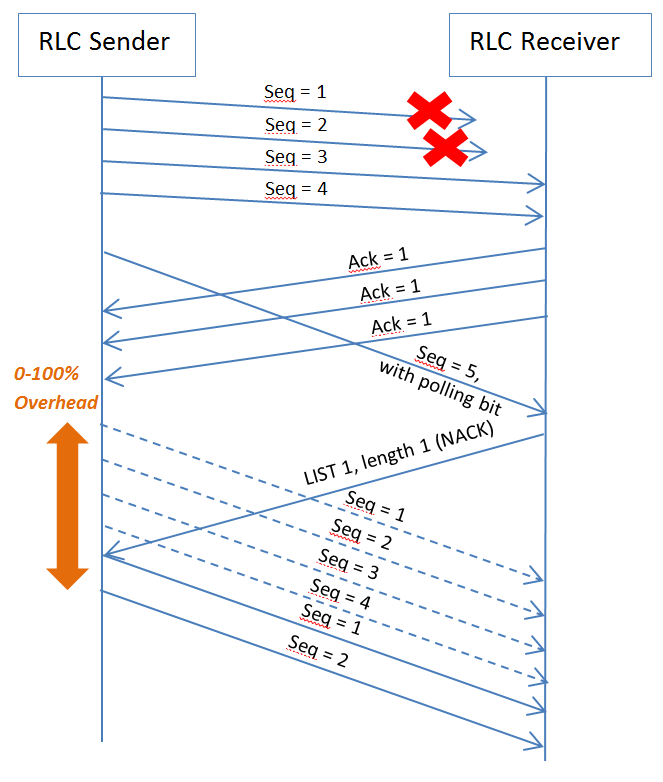
\includegraphics[width=0.45\textwidth]{figs/Draw.png}
\caption{Draw Minus: the predication accuracy is less than 50\%}
\label{fig:draw.minus}
\end{figure}

\begin{figure}
\centering
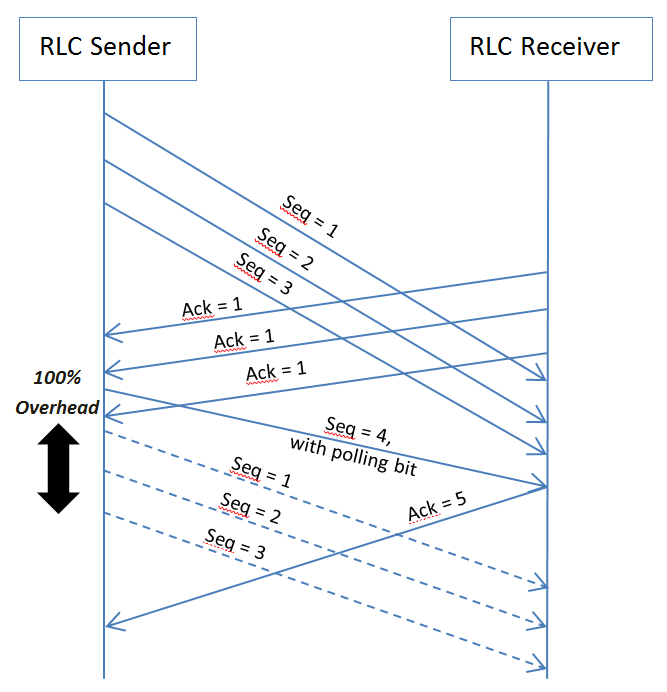
\includegraphics[width=0.45\textwidth]{figs/Loss.png}
\caption{Loss: all predications fail}
\label{fig:loss}
\end{figure}

% Cost-Benefit Table
\begin{table}
\begin{tabularx}{0.48\textwidth}{ | c | X |}
	\hline
	\textbf{Case Name} & \textbf{Percentage of Occurrence (\%)} \\
	\hline\hline
  	Win & 10.32$\pm$1.89 \\
  	\hline
  	Draw\_{Plus}* & 64.68$\pm$8.32 \\
  	\hline
  	Draw\_{Minus} & 20.63$\pm$3.45 \\
  	\hline
  	Loss & 4.25$\pm$0.06 \\
  	\hline
\end{tabularx}
* The Draw\_{Plus} case excludes the percentage of Win
\caption{The RLC Fast Re-Tx Cost-Benefit Table}
\label{tab:rlc.fast.sim}
\end{table}


\label{sec:eval}

          % 4.0 pg
\section{Discussion}

\subsection{Future Work}
The current study is primarily focus on the latency improve over the RLC layer. It is also possible to measure the delay improvement over application layer directly, especially for the initial period of the data transmission. Another possible direction is to evaluation the energy efficiency for the improved RLC protocols with fast retransmission mechanism. Since QxDM provides device data transmission power information, we could also evaluate the energy saving over each RRC state and state transitions.

\subsection{Limitation}
Since we could not modify the handset's NIC (network interface card) driver, we only evaluate the modified trace information based on the QxDM traces. Currently we assume the fast retransmitted RLC PDUs guarantee to be received on the base station, but the actual channel is lossy and the actual benefit might be lower than the simulated results. In addition, since the modification of RLC protocol requires hardware modification, the deployment of the modified protocol could be slower than a software solution.

\label{sec:disc}


          % 0.5 pg
\section{Related Work}

One of the previous cross layer study combined inferred RRC state information with collected device power trace to imply application behaviors leading to unnecessary energy consumption~\cite{aro}. Their primarily focus on the application level energy optimization instead of latency. The QxDM in our study provides more fine grained performance, latency and power information. We could have more detailed insights to understand data link layer root cause for abnormal latency and inefficient energy consumption behaviors in upper layer. 

Related to our RLC fast retransmission proposal, a previous study provides cross comparison analysis over the TCP and RLC protocols, and optimizes the default protocol parameters~\cite{opt.tcp.rlc}. Their primary goal is to improve the performance behavior by introducing TCP congestion control mechanism into the RLC layer. However, their traces are purely generated from simulation software, whereas we use real traffic traces.

\label{sec:related}       % 2.0 pg
\section{Conclusions}
\label{sec:conc}

From the RRC state inference model, we evaluated the latency across each RRC state and state transitions. We observed the extra latency in the FACH state using RRC inference methodology. Utilizing the QxDM monitoring tool, we have a better visibility over RLC layer traffic information. We wrote a QxDM log parser and analyzer to cross mapping the transport layer and data link layer information, and identified the root cause of abnormal delays cause by the imperfection in the RLC layer protocol. We proposed a RLC \textit{Fast Re-Tx} mechanism to actively response to the PDU loss, and evaluated the delay cost-benefit over real-time traces. The latency reduction is up to 35.69\% over FACH state, and it could also reduce the overall latency by 2.66\%. Therefore, the RLC \textit{Fast Re-Tx} mechanism could enhance the user mobile experience by introducing less delays, especially during the initial data transmission period.
          % 0.25 pg
\section{Acknowledgments}

We would like to thank Yihua Guo, Sanae Rosen, and Z. Morley Mao for supporting and commenting on this paper.

\label{sec:ack}


           % 0.25 pg

%Uncomment this line if your paper has / uses end notes
%\theendnotes

%\footnotesize
\raggedright
\sloppy
\bibliographystyle{abbrv}
\bibliography{bib}


\end{document}

